\documentclass[aps,prb,twocolumn,groupedaddress,nofootinbib,floatfix]{revtex4-1}
%
\usepackage[hyperindex,breaklinks]{hyperref}
\usepackage{amsmath,amsfonts,amssymb,amsthm,bm,caption}
\usepackage{calc,ifthen,natbib,graphicx,gensymb,chngcntr}

\newcommand{\beq}{\begin{equation}}
\newcommand{\eeq}{\end{equation}}
\newcommand{\ben}{\begin{enumerate}}
\newcommand{\een}{\end{enumerate}}

\newcounter{captionedequationset} %numbering
\newdimen\captionlength
\newcommand{\eqcap}[1]{
    \refstepcounter{captionedequationset}% Step counter
    \setlength{\captionlength}{\widthof{#1}} %
    \addtolength{\captionlength}{\widthof{Equation set~\thecaptionedequationset: }}
    %If the caption is shorter than the line width then
    % the caption is centred, otherwise is flushed left.
    \ifthenelse{\lengthtest{\captionlength < \linewidth }} %
    {\begin{center}
            Equation set~\thecaptionedequationset: #1
        \end{center}} 
    { \begin{flushleft} 
        Equation set~\thecaptionedequationset: #1 %
        \end{flushleft}}}

%\setlength{\skip\footins}{0.3in}
\begin{document}
%
\title{Data Mining the Gaia Archive to Uncover the Secrets of Stellar Clusters}

%
\author{William Wainwright}
%
% DON'T CHANGE ANYTHING IN THE NEXT FEW LINES OR DELETE BLANK LINES
%
\affiliation{This work was submitted as part of a course requirement for completion of the BS degree in the Physics Program at RIT and, in its current form, does not appear in any publication external to RIT.}
%
% PUT YOUR ADVISOR NAME BELOW.  DON'T DELETE ANY LINES
%
\altaffiliation [Rochester Institute of Technology, School of Physics and Astronomy, Faculty Advisor: ]{Dr. Michael Richmond}

\date{\today}

\begin{abstract} The Gaia-DR2 data release includes photometric measurements of over a billion stars in the Milky Way. Using these measurements, I have been able to robustly filter out and select for members of stellar clusters. I have been able to apply methods of data reduction and fitting to match theoretical isochrones to the color magnitude diagrams produced for these clusters. Through selective, sequential fitting, I have been able to determine the age, metallicity, and reddening of the cluster M67, and have thus far filtered and approximately fit the cluster M35. The best fit determined for M67 was as follows: $\left[\frac{Fe}{H}\right]\approx -0.5$, $\left[\frac{\alpha}{Fe}\right]\approx 0.2$, $\text{Reddening } E\left(BP-RP\right)\approx 0.05$, $\text{Age}\approx 4.5 \text{ Gyr}$. Uncertainties are bounded by the intervals provided in the isochrones.
\end{abstract}

\maketitle

\section*{Introduction}
The primary tool for categorizing the evolution and distribution of stars is the Hertzsprung-Russel (HR) diagram. The simplest way to construct an HR diagram is to observe a cluster of stars, and plot the apparent magnitude of the stars versus their color index. The primary characteristic of a color-magnitude diagram(CMD) is called the main sequence. The main sequence represents a generally linear section of the CMD where stars of different composition spend most of their life. Where most of the interesting physics happens, however, are the locations away from the main sequence, such as the main sequence turnoff. By analyzing measured properties and the relationships between them of the stars in these supplementary regions, we can glean insight about unmeasured properties of the stars and the clusters to which they belong.

\section*{Gaia Instrumentation}
The Gaia spacecraft is a space observatory that was launched by the European Space Agency (ESA) in late 2013.``The main goal of the Gaia mission is to make the largest, most precise three-dimensional map of our Galaxy by surveying an unprecedented one per cent of the galaxy's population of 100 billion stars''\protect\cite{ESA}. Gaia is located approximately 1.5 million kilometers from the Earth, in the Earth-Sun L2 Lagrange point\protect\cite{ESA}. The Gaia spacecraft is designed for astrometry, and measures the position, proper motion, color index, and apparent magnitude of stars in addition to other astrometric properties. Gaia has measured each of its targets over 70 times through its current 5 year mission length, and will continue to observe targets through its extended lifetime due to low fuel usage\protect\cite{ESA}. 

Gaia observes two patches of the sky concurrently. The light from two openings is focused onto the most powerful camera ever flown in space, with 106 CCDs and almost 1 billion pixels\protect\cite{GaiaSpec}. The CCD array is segmented into different regions, which each independently measure their respective astrometric variables. On average, Gaia records the astrometric data for two million stars per hour\protect\cite{GaiaSpec}. So far, the Gaia mission has resulted in two bulk data releases. These Gaia data releases have been made available to the public through the ESA Gaia archive\protect\cite{GaiaData}. The Gaia data releases have allowed for researchers to computationally examine the data in a wide variety of fields. The second data release (DR2) of the ESA Gaia mission provides the position, proper motion, parallax, color, and magnitude of over a billion stars among other properties. The unprecedented breadth and precision of the Gaia survey makes possible an innumerable number of computational analyses of the data, and to a degree of precision previously impossible.

The primary astrometric  variables that Gaia measures are the position, parallax, apparent magnitudes in various filters, and proper motion. The position is measured in right ascension (RA) and declination (DEC). These measurements give a unique address to each star irrespective of geographic location and time. The parallax is a measurement of the apparent angular shift of an object in the sky due to Earth's motion around the sun. The inverse of the parallax angle in arc seconds is the distance to the object in parsecs. The magnitude is a measurement of light intensity, and can be measured in different filters to get an idea of how bright the object appears in different wavelengths of light. By subtracting the magnitude of the object in different filters, we get a value known as the color index, which represents how red or how blue a source is. The magnitude scale is logarithmic and inverse, so a smaller magnitude represents a brighter target. Proper motion is a measurement of how an object appears to move across the sky in a plane tangential to the line of observation. The measurement of how an object moves along the line of sight is the called radial velocity. Proper motion is typically measured in terms of motion in the RA and DEC separately.

Despite Gaia's impact and importance, the data produced by the Gaia mission has a few pitfalls and caveats. One issue with Gaia is that the radial velocities calculations were 'contaminated' for a majority of stars in close proximity to other stars. Unfortunately, this means that when looking at stellar clusters, the radial velocity measurements are few and far between. One of Gaia's greatest advancements is the increased precision of trigonometric parallax measurements and wider scope of stars compared to its predecessor, Hipparcos. The uncertainty in parallax tends to increase with distance, however. As a result, many of the stars at greater distances from Earth have several percent uncertainty in their measurements. Measurements of apparent magnitude and color index cannot necessarily be taken at face value, either. Gas and dust between the observed star and Earth can absorb and scatter some light, leading to a reduction in observed brightness known as extinction. Dust can also preferentially scatter blue light, leading a star to appear more red by virtue of a higher portion of the red wavelengths reaching Gaia. This phenomenon is accordingly called interstellar reddening.


\section*{Programming Framework}
In order to analyze Gaia data, I first created a code framework to read in data from comma separated value (CSV) files and store the parameters in memory in an efficient way. When processing a new cluster, I first download a CSV file from Gaia of all of the stars within a radius of the supposed center of the clusters I am looking at. I read in the data from the CSV file and create a two dimensional array of values where each row is a star and each column is a measurement. Since managing arbitrary header IDs isn't particularly human friendly, I then store each star's information in a class object. These class objects allow me to create variable names associated with each star, so that I can specifically call for the properties by name when analyzing the data. I store a list of all of the star objects from the CSV file in a stellar cluster class object, along with a few calculated parameters about the cluster.

In order to allow for meaningful processing of the data based on astrometric measurements, I remove any stars from the list that do not have a valid numerical measurement for any of the variables I control for. Therefore, any star without a measurement for RA, DEC, proper motion, apparent magnitude, or color index measurements is removed from the list before any further processing is done. I also calculate basic statistics about the stars in the field and remove any egregious outliers that are more than several standard deviations from the mean proper motion of the entire data set. Because the stars along a given line of sight have a generally large spread in measurements, filtering in this way serves to remove only a handful of extreme outliers.


\section*{Filtering}
Before any meaningful analysis of a cluster can take place, it is necessary to identify what stars are members of a cluster in question rather than foreground or background contamination. Because Gaia makes available a multitude of astrometric measurements, it can be difficult to ascertain what properties of a given star are relevant in this determination. In order to investigate what properties are relevant to filtering, I created a series of plots in different parameter spaces to try and identify any notable features by eye. It became almost immediately apparent that proper motion was one of the key parameters, as when plotting proper motion in RA versus proper motion in DEC, a tight clumping of points is apparent. My most robust method of filtering thus far has therefore been to manually define a radius of tolerance around this clump in the proper motion space, and reject any stars that do not fall within this circle as outliers.

\begin{figure}[!h]
	\centering
      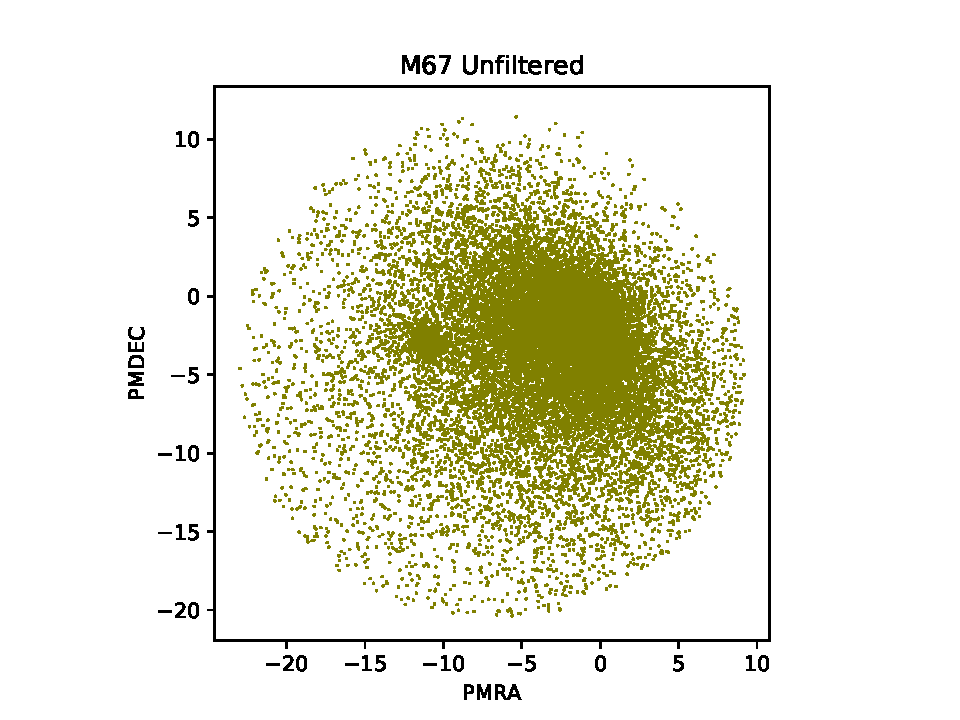
\includegraphics[width=4in]{M67_pm_unfiltered.pdf}
	\caption{Plot of the proper motion in the DEC versus proper motion in the RA for M67. The tight clumping left of center is the region that is selected when filtering. Stars outside of this region are considered contamination}
	\label{fig:M67_pos}
\end{figure}


\begin{figure}[!h]
	\centering
      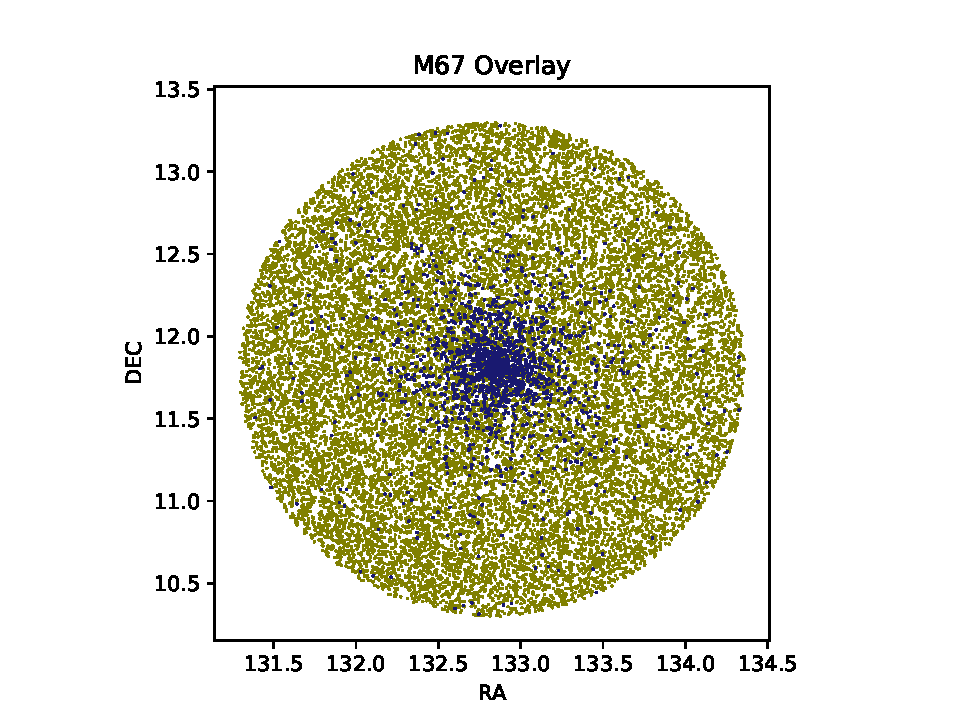
\includegraphics[width=4in]{M67_ra_dec_overlay.pdf}
	\caption{Plot of the declination versus the right ascension for a 1.5 degree radius around M67. Blue points represent members of the cluster post-filtering, and green points represent stars that have been filtered out.}
	\label{fig:M67_pos}
\end{figure}

Often the proper motion filtering is not enough, however, and I have found that filtering by removing stars which are more than a few standard deviations outside the mean parallax is an effective supplementary step in filtering. Theoretically, filtering by radial velocity in addition to proper motion would help to effectively remove a vast majority of contamination. However, because stars in a cluster are generally in close proximity, Gaia does not have uncontaminated radial velocity measurements for a vast majority of the stars in the selected line of sight. After all of the filtering, I typically reduce a data set on the order of 20-50 thousand stars to a few thousand.

\section*{Color Magnitude Diagrams}
A valid question to have at this point is ``How do I know whether my filtering method is effective?''; This is where color magnitude diagrams come in. One of the main features of a CMD is the main sequence. The main sequence is a generally linear region of the diagram where stars `live' for a majority of their lifetime. This is to say that when plotting measured values of apparent magnitude and color index, properties which change depend on the composition and age of the star, the data point will generally end up on the main sequence for most of a star's lifetime. At one end of the main sequence is the main sequence turnoff. This feature of the diagram usually appears to curl back over the main sequence, and represents data points for stars that are in the late stages of their lives, typically undergoing a drastic change in internal fusion dynamics. 

The lifetime of many of these stars is on the order of billions of years, so we are unable to measure a star over time and watch is evolve up the main sequence. In order to construct a real life CMD, we can cheat by plotting a bunch of stars that formed at the same time. Generally, higher mass stars will evolve and die off more quickly. Because of this, even if the less massive stars have not had time to evolve up and off of the main sequence, there will still be stars that are present in our measurements to map out the majority of the main sequence and main sequence turnoff. What this means is that we can use how well the main sequence and turnoff are preserved as a proxy for how good of a filter we have.

Plotting a CMD for the unfiltered data along a given line of sight produces an unintelligible blob of data points, as seen in Figure \ref{fig:M67_CMD_unfiltered}. After filtering by proper motion and parallax, however, a clear main sequence and turnoff become apparent, as seen in Figure \ref{fig:M67_CMD_filtered}. All determinations I have made in the effectiveness of various filtering techniques have come from meaningful differences in the post-filtering CMD. Though filtering by these parameters is effective, a fine balance needs to be maintained between filtering out non-members and erroneously filtering out members.

\begin{figure}[!h]
	\centering
      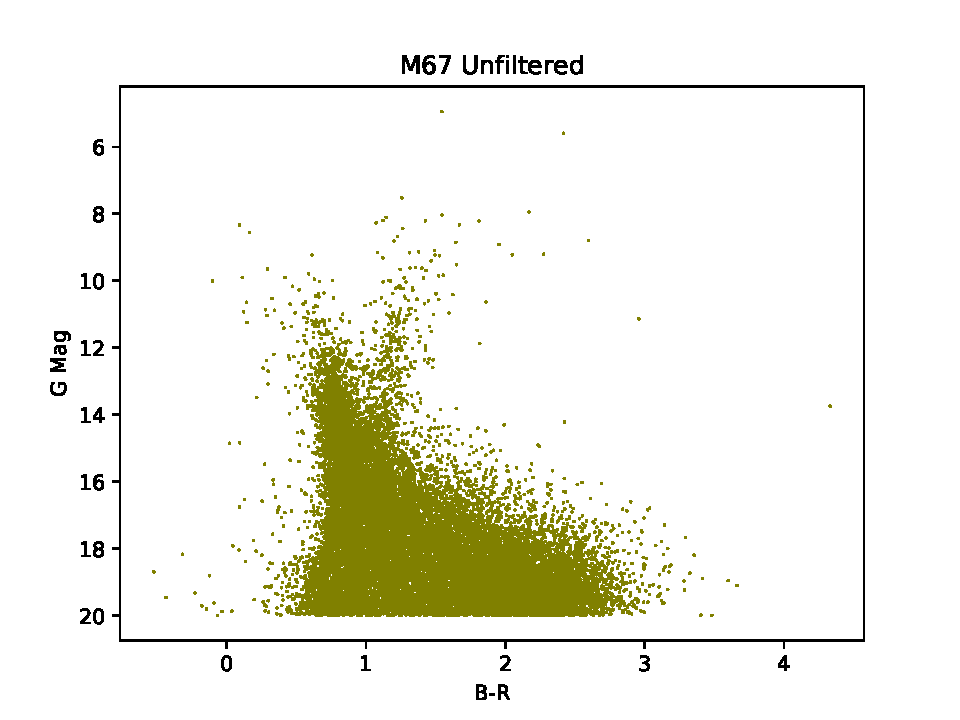
\includegraphics[width=3.5in]{M67_CMD_unfiltered.pdf}
	\caption{Color-Magnitude diagram of stars in M67 generated using unfiltered data from Gaia DR2.}
	\label{fig:M67_CMD_unfiltered}
\end{figure}

\begin{figure}[!h]
	\centering
      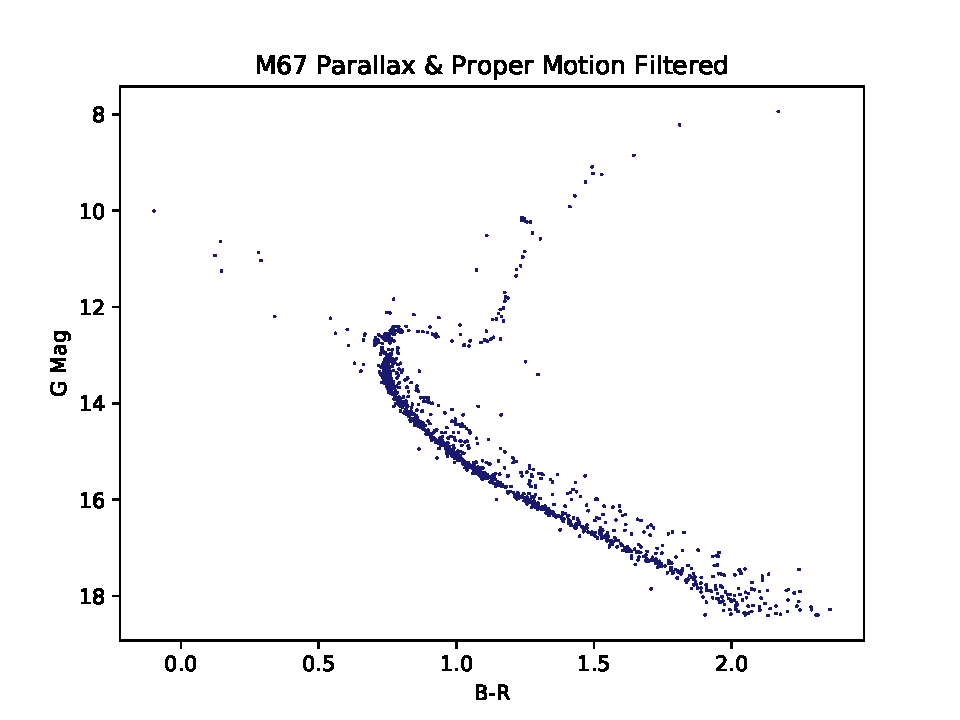
\includegraphics[width=3.5in]{M67_CMD_filtered.pdf}
	\caption{Color-Magnitude diagram of stars in M67 generated using filtered data from Gaia DR2. Many of the supplementary features mentioned are present on the plot, including a secondary main sequence, red clumping, and blue stragglers.}
	\label{fig:M67_CMD_filtered}
\end{figure}

Visible on the the CMD for the cluster M67, as seen is Figure \ref{fig:M67_CMD_filtered}, are a few additional features. A less dense string of stars, called blue stragglers, appears to continue the main sequence trend line past the main sequence turnoff point. The exact origin of these blue stragglers is not known, but the most plausible explanation is that these stars formed later than the majority of the stars in the cluster. It is also possible that these blue stragglers are the result of stellar collisions. Another feature visible on the CMD for M67 is a phenomenon known as red clumping. In contrast to the relatively sparse data points past the main sequence turnoff point, there are a dense clumping of data points at one particular segment of the post turnoff region. The reason for this clumping is that when lower mass stars are evolving off of the main sequence, their hydrogen core has fused into a core of helium. Stars build up a core of helium until a point where the conditions are right for helium fusion to spontaneously begin, known as a helium flash. Stars tend to spend a longer time in the helium fusing stage compared to other stages past the main sequence, causing a higher density of points on the CMD.

Also of note on the CMD for M67 when compared to a theoretical main sequence, is that the main sequence has a spread to it. The dimmer edge of the main sequence is relatively well defined and dense. Conversely, the the brighter edge of the main sequence line is less well defined and the space above the dimmer edge is considerably less data point dense. I believe the reason for this phenomenon is due to the presence of binary stars. Binary stars are a system of two stars that are orbiting close to each other, and are therefore often observed as a single point source star. If two stars orbiting each other had roughly the same color index and magnitude, then when they are observed side by side relative to the line of sight, they would appear twice as bright as a single star with the same color index on the main sequence. As the stars orbit, they would reach a minimum brightness of that of a single star of that color index, with one star behind the other. Any combination of stars between these two states, with partial eclipsing, or stars of unequal color or magnitude, would produce the spread of points seen between these two edges. Therefore, I believe that the more dense bottom edge is made up of single and eclipsing binary stars, while the upper edge and the spread between is comprised of binary stars of some description. In order to confirm this, I fit two lines to a segment of the main sequence with identical slope, one line to each edge of the main sequence. Magnitude is logarithmic, so a doubling in brightness would correspond to a 0.75 magnitude shift. I found that the lower and upper edges of the main sequence to be between 0.7 and 0.8 magnitudes apart, helping to solidify this idea. The formula for converting from intensity to magnitude is $m_1-m_2 = -2.5\text{log}\left(\frac{I_1}{I_2}\right)$


\section*{Isochrones}
Once I have a reasonably robust list of stellar cluster members, I can then try to determine some parameters of the cluster. I mentioned before that the age and composition of a group of stars needs to be similar in order for the main sequence to take shape. Because of this, we can infer properties about the age and composition of the cluster, whose members construct a connected main sequence. In astronomy, metallicity is a measure of the ratio of certain elements compared to the hydrogen and helium in a star. Metallicity is an important factor in studying larger scale stellar population evolution, because an older population of stars tends to have a lower metallicity than a younger population of stars. Measuring the age of the cluster also helps to confirm this relationship and further constrains stellar population evolution models.

By now, astronomers have a pretty good model for how typical stars evolve throughout their lifetime. Samples of model star data with a given age and metallicity are used to produce theoretical CMDs called isochrones. By comparing a series of isochrones to the cluster data and determining the goodness of fit, I am able to infer the age and metallicity of the cluster. A sample of a few different isochrones can be seen in Figure \ref{fig:Isochrone_Sample_Age} and Figure \ref{fig:Isochrone_Sample_Metallicity}. It is important to note that changes in metallicity tend to shift the isochrone horizontally, and changes in age shift the turnoff point further down the main sequence, towards the dimmer and redder stars. A further complication, however, is that interstellar reddening shifts the isochrone horizontally, and extinction shifts the isochrone vertically. Reddening and extinction are coupled proportionally, but without spectra to determine what color the star should be, it is difficult to properly identify the reddening.

\begin{figure}[!h]
	\centering
      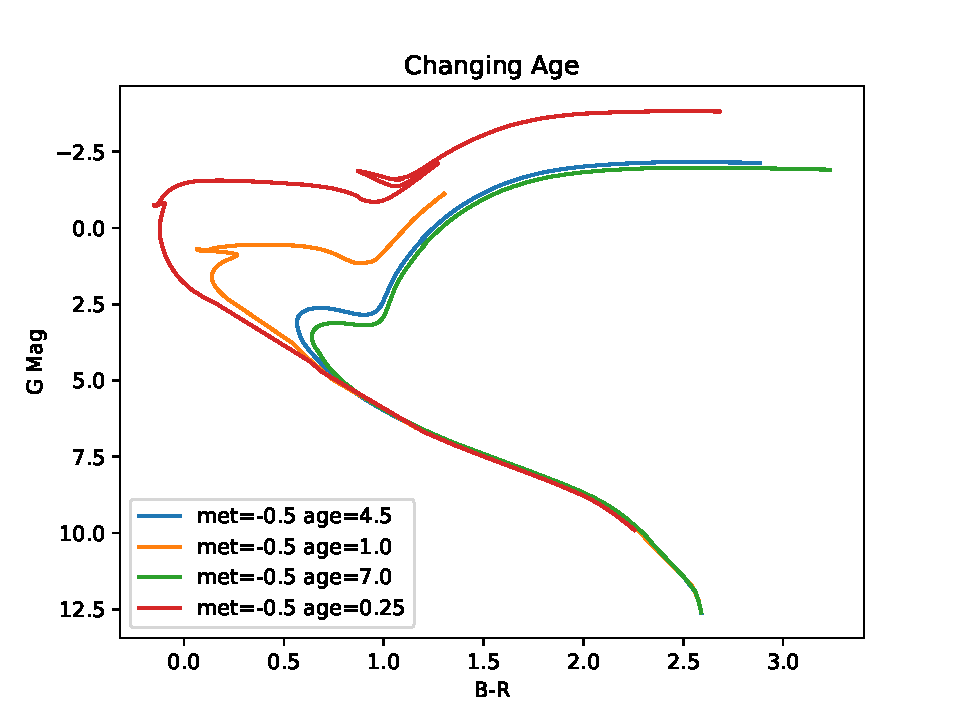
\includegraphics[width=3.5in]{iso_sample_age.pdf}
	\caption{Color-Magnitude diagram of various isochrones with a spread of ages in billions of years and the same metallicity.}
	\label{fig:Isochrone_Sample_Age}
\end{figure}

\begin{figure}[!h]
	\centering
      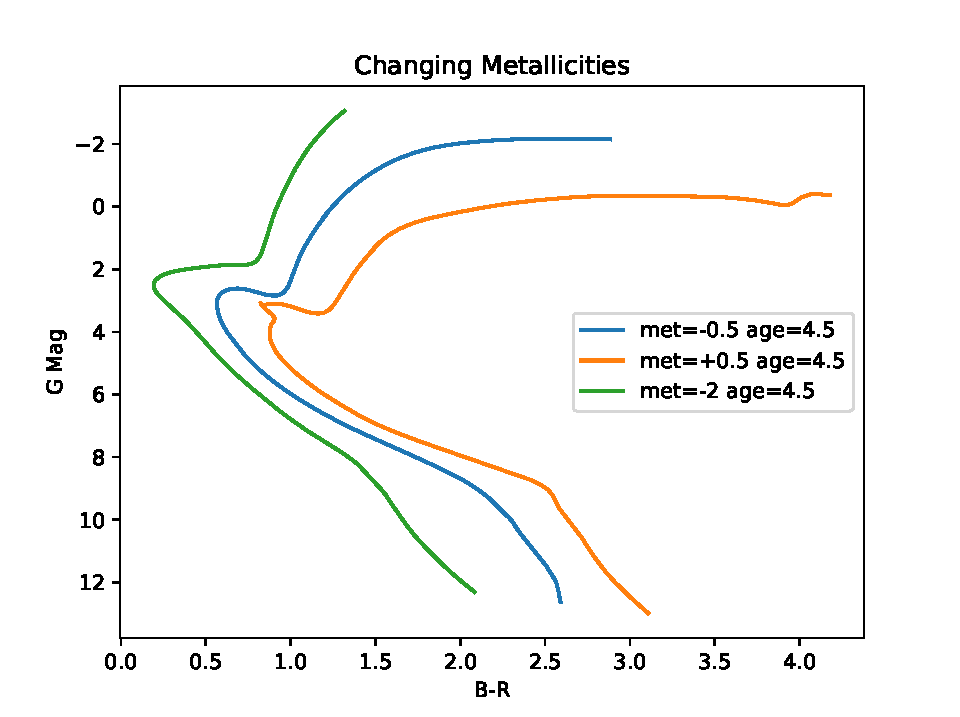
\includegraphics[width=3.5in]{iso_sample_metallicity.pdf}
	\caption{Color-Magnitude diagram of various isochrones with a spread of $\frac{Fe}{H}$ metallicities and the same age.}
	\label{fig:Isochrone_Sample_Metallicity}
\end{figure}

\section*{Fitting}
To fit the data from the clusters I have processed, I used isochrones provided by Dartmouth University's Stellar Evolution Database\protect{\cite{Isochrones}}. The isochrones are provided in steps of 250 million years, with a spread of values for metallicity in terms of both $\frac{Fe}{H}$ and $\frac{\alpha}{Fe}$. In other words, the fraction of iron to hydrogen, and of ``alpha'' to iron. Alpha includes elements fused from helium nuclei, such as oxygen and silicon.

I have tried a few different methods of determining the best fit between the isochrone and the cluster data. The obvious, brute force method is to calculate the distance between every star and the isochrone and try to minimize the mean of these distance. Two issues arise with this approach. The first issue is that, depending on the number of stars left after filtering, the computational time required to determine this value is long. If your goal is to test several thousand isochrones to determine the best fit, then the computational time is prohibitively long. The other issue with this method is that there are a lot more points in the main sequence than past the main sequence. As a result, this method means you are selecting for isochrones that most closely match the main sequence, even at the cost of missing the post turnoff stars completely.

In order to account for the issues in statistical weight of the post main sequence turnoff stars, as well as the computational overhead, I condensed the data set into a spatially representative but statistically unrepresentative set of point. I segmented the CMD into vertically stacked slices, and took the median color index and magnitude in those bins to be a single point. The result of this is that a span of one magnitude in the main sequence is made up of roughly the same number of points as a one magnitude span post main sequence. This condensing of points serves to reduce the computational time drastically as well as to weigh the importance of the turnoff fit equally with the main sequence fit.

With the points condensed, I then fit the best isochrone by attempting to minimize the value:
\beq
\frac{1}{N}\sum\limits_{n=1}^{N}\sqrt{\left(x_n-x_{iso}\right)^2+\left(y_n-y_{iso}\right)^2}
\eeq
where $x_n$ and $y_n$ are a given condensed point's color index and G-band magnitude, $x_{iso}$ and $y_{iso}$ are the coordinates of the closest isochrone point, and $N$ is the total number of stars. In other words, I am trying to minimize the mean distance between the condensed points and their closest isochrone points. The results of the fit to M67 can be seen in Figure \ref{fig:M67_iso_best_fit}.

\begin{figure}[!h]
	\centering
      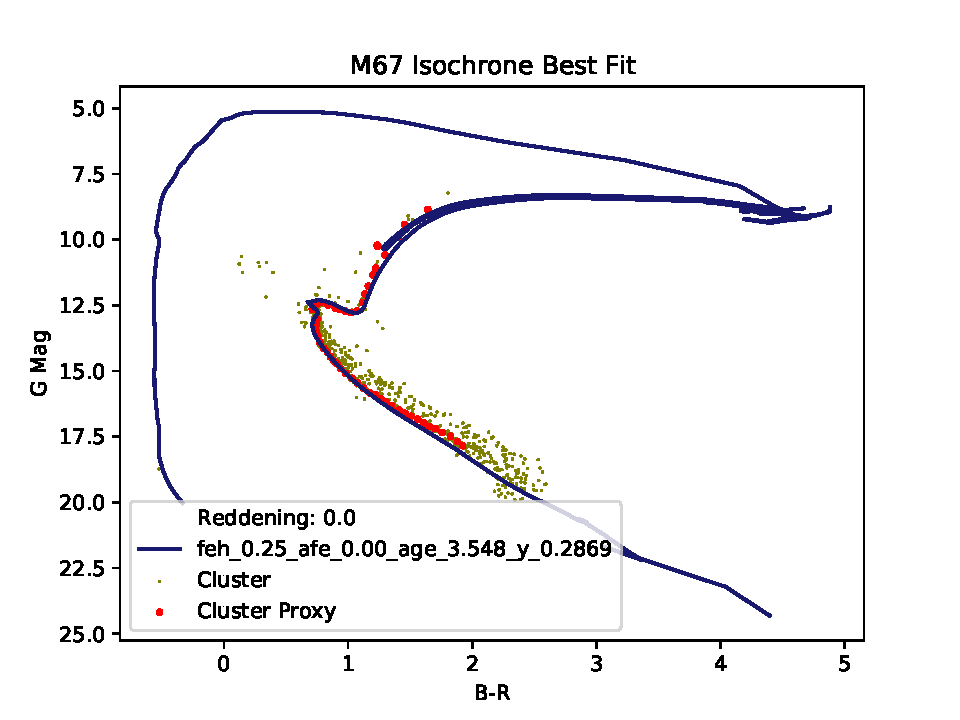
\includegraphics[width=3.5in]{M67_CMD_Iso_BestFit.pdf}
	\caption{Color-Magnitude diagram of the stars in M67 with an overlaid best-fitting isochrone. The red points represent the condensed points to which the blue isochrone was actually fit.}
	\label{fig:M67_iso_best_fit}
\end{figure}


I originally chose M67 because it is believed to have a reddening that is fairly negligible. As a result, I could focus on fitting the isochrones to M67 without having to account for reddening. When it comes to other clusters, however, the reddening can impact the fit drastically, leaving me with three options. I could cite literature and hard code values for the reddening in for a given cluster, read in reddening information from Gaia, or process only clusters with known, negligible reddening. The Gaia measurements for reddening are sparse and seemingly inaccurate, so that left me with two choices. I chose to do none of these options, and instead sequentially determined the best fit for a whole series of reddening values. While the plausibility of this method seems a bit dubious, the results thus far seem promising. I am still in the process of tweaking the filtering and fitting methods for clusters with non-negligible reddening, however, so the efficacy of the sequential fitting method remains to be determined.


\section*{Conclusion}
The results of the filtering and fitting methods applied to M67 are extremely promising. By eye, the fit of the isochrone to the cluster data is superb, and the values determined for the reddening and age of M67 agree within uncertainty to those of Yadav et al\protect{\cite{Yadav}}. To some extent, the uncertainty of fitting is limited by the isochrones, which are only available in age intervals of 250 million years and sporadic metallicities. Though the fitting for M35 and other non-negligible reddening clusters is still a work in progress, the results thus far are promising and give hope of a robust, versatile filtering and fitting method for a vast swathe of stellar clusters in the Milky Way.

\section*{Capstone II}
There are a few different avenues that I could take this project in the second semester of capstone. The obvious next step is to perfect the filtering and fitting techniques applied to M67 and M35. One next step I intend to incorporate is to replace the manual defining of a proper motion threshold with an unsupervised nearest neighbors algorithm. This algorithm should be able to find clumping in the data, and will hopefully be able to identify clumping in the proper motion space. Should the automatic clump finding method not work out, I would still be able to continue while manually defining the radius threshold for each cluster, but it would limit the scope of how many clusters I can process and characterize.

After that, the directions the project can take really open up. I could, for example, turn the algorithm loose on arbitrary patches of the sky, seeing if the code can find and characterize a cluster along that line of sight. This could potentially lead to the identification of unknown clusters, or just reaffirmation and further constraining of the age, metallicity, and reddening for known clusters. Another possibility is using the refined method of filtering to investigate cluster membership as a function of physical radius. This line of study would relate to topics like cluster evaporation and n-body dynamics. A third option is to spend the rest of capstone II fine tuning the fitting and filtering methods, providing robust error and uncertainty calculations and making more of a methods type paper about the process. Regardless of the direction this project takes, I am excited to spend another semester exploring the stars.

\begin{acknowledgments}
I would like to thank my advisor, Dr. Richmond, as well as Dr. Bhattacharya, the capstone committee, and the RIT School of Physics and Astronomy.
\end{acknowledgments}
%
%change the name of the bibliography file to your own name
%make sure you have h-physrev5.bst file in the same directory as your tex file and bib file
%then compile using Latex-Bibtex-Latex-Latex sequence!
%

\bibliographystyle{h-physrev5}
%Note that it does not need the .bib extension in this line!
\bibliography{Wainwright_Capstone_I}

\end{document}

